\section{Preliminary Designs} 
\label{sec:preliminary_designs}

In the course of research and discussions about possible visualization to implement for our project, we came up with a number of suitable visualizations that seemed suitable to use in our project. Below is the list and description of each visualization along with reasoning to support our choice of this visualization.

\subsection{Pick-Up vs Drop-Off}
\label{sec:viz1}

The first design we thought of was a geographical map which plots the arrival and departure areas of the share-bikes and maps this data according to their frequency. So, for this visualization, a geometrical plot was being used. Here the marks were the share-bikes (either arriving or departing) and the attribute was the frequency of arrival or departure. We planned on using circles to denote the arrival or departure at the bike station. This way, the mark of the visualization could be considered as a circle. Since we will be mapping both the arriving and departing bikes, it would be confusing to have circles of both types of data of the same color. Hence, we decided to denote departing and arriving bikes by red and blue color respectively. Similarly, the frequency of arrival/departure would be encoded by the area of the circle (encoding rule). The channels here are the geographical (x and y) positions, color and area. 

This choice of visualization was directly influenced by similar work \cite{UrbanDataCyclist} done by Daniel Peterson, where they mapped hires and drop-offs on a location with circles and encoded the frequency with the area of the circle. The following design is from the above-mentioned study itself.
\begin{figure}[h]
	\centering % avoid the use of \begin{center}...\end{center} and use \centering instead (more compact)
	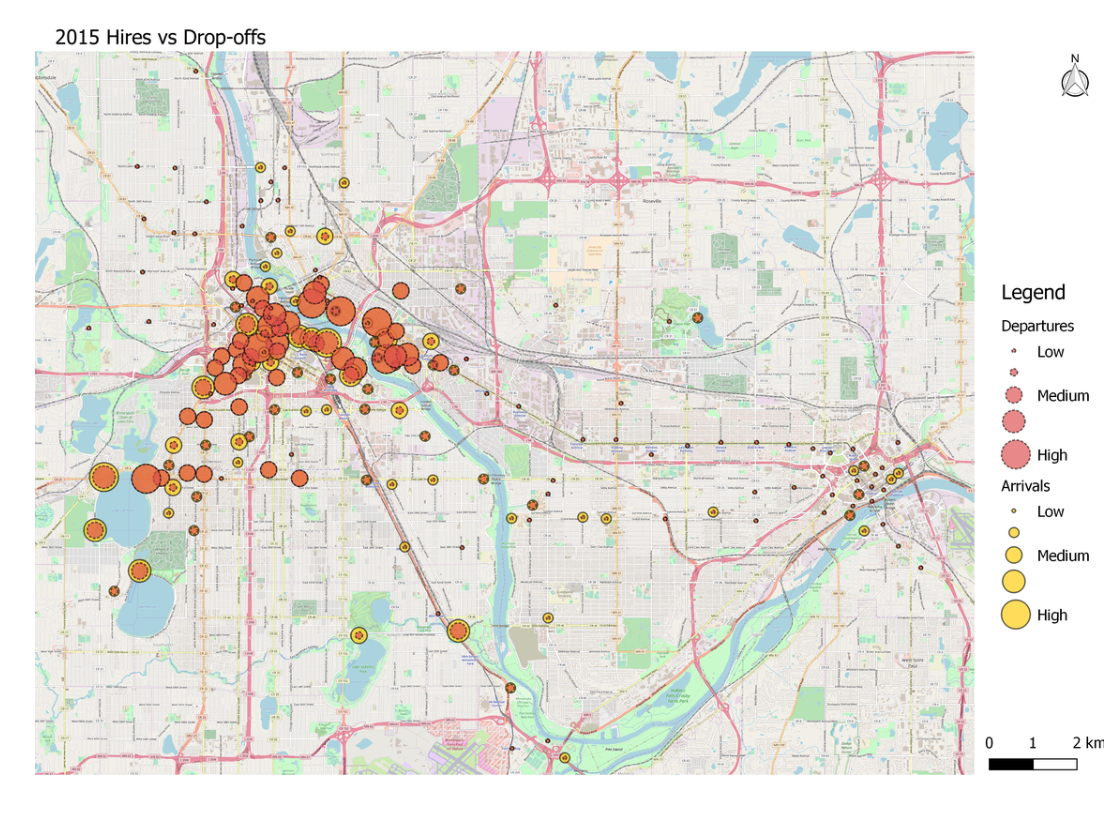
\includegraphics[scale=0.36]{figs/first_viz.PNG}
	\caption{\footnotesize{Mapping hires and drop-offs by circle area. \cite{UrbanDataCyclist}}}
	\label{fig:First viz Chart}
	\captionsetup{justification=centering,margin=1cm}
	\vspace{-10pt}
\end{figure}
\newline
This choice of visualization adheres with much of the design principles studied in our class. It follows the principle of effectiveness as the data is easily separable. By using a single channel (color) to distinguish between hires and drop-offs of bikes is more effective than using 2 channels for it. Also, we were planning to make this an unconstrained navigation which allows more freedom to the user to navigate. On the topic of task abstraction, this visualization is suitable to locate areas of high business activity. The area of circle directly correlates with the idea of high business volume.

In addition to that, the choice of color itself (red and blue) are easy to distinguish and hence are easily separable. These colors do not generally mesh with the mostly green and gray geographical background as well. This choice of visualization helps in the comparison between the hire data and drop-off data. In addition to that, it also helps in comparing the same kind of data (hires or drop-offs) with each other based on different locations. One drawback of this visualization is that the area of the circle does not give a quantitative value of the frequency of hires/drop-offs from the visualization itself. 

\subsection{PassType Mapping with Time}
\label{sec:viz2}

One of the things we were interested in the bike-sharing data was analyzing the bike pass types and their trend. For the bike-sharing service we chose, there are 3 kinds of passes -- daily, monthly and annual. Analysis of these bike-passes with a time of different granularity was not found in other visualization projects and research papers. This encouraged us to take on this concept to find some pattern or trend with this data. 

For this visualization, we planned on using line graph how the number of passes of each kind being bought for different levels of time granularity. The granularity levels could be a month, quarter or year. This option could be selected by the user from a drop-down box to the right of the line graph. Within the line graph, three lines represented the three types of passes. The choice of colors was red, blue and green. This triplet of colors form the basis of the RGB-colorspace which goes to prove that they are distinct from one another when used together. 

The X-axis would be the time axis and the Y-axis would be the magnitude axis. Here, the task abstraction shifts more towards the discovering and analyzing side. Our aim was to find some sort of trend moving forward with time. We expected to see an increase in monthly passes and a slight increase in annual passes. This would indicate that the bike-sharing service is getting popular with time. A more visible change could be perceived if the time was on a level of the year. On the other hand, the daily passes data would give a whole different perspective on how people use these services. By generalizing weather over months i.e. December-March for Winter, we could check if fewer people use the service during winters and more during spring/summer. 

In addition to the task abstraction, this visualization followed the principles of effectiveness and expressiveness as well. It is clearly distinguishable and it encodes only the required values. Being line graph, the level of accuracy is pretty good. Here, we have applied the principle of superimposing by overlaying the line graph of all 3 pass types into a single chart. Our assumption was that this number of overlay won't harm the distinguishability of the lines. Allowing the user to change the time granularity also helps in bringing user interactiveness into the picture. A rough sketch of what the visualization would probably look like is given below:
\begin{figure}[h]
	\centering % avoid the use of \begin{center}...\end{center} and use \centering instead (more compact)
	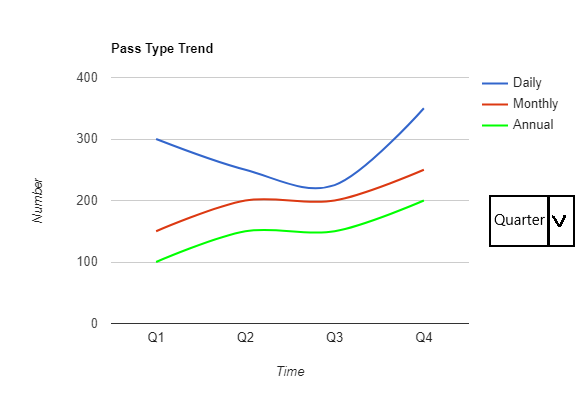
\includegraphics[scale=0.45]{figs/bar-graph.png}
	\caption{\footnotesize{Mapping of pass type with time granularity}}
	\label{fig:Second viz Chart}
	\captionsetup{justification=centering,margin=1cm}
	\vspace{-10pt}
\end{figure}
\newline

\subsection{Crossfilter Based Geographic Mapping}
\label{sec:viz3}

For the final design, we thought of implementing a crossfilter enabled geographic mapping of data. Basically, we will be expanding on the first visualization choice in this list. The difference here is that in the first visualization, the time range has been fixed beforehand. So there is no user interactivity in that visualization. On the other hand, this visualization adds a dynamic element to the previous static visualization. Here, we will have a geographic map just as in the first choice. We plan on mapping the drop-offs and hires just like in the first visualization. The data represented in the geographic plane can be controlled by a slider that can move through a time histogram. The time histogram will map the average duration of a trip for that period of time. So in this way, we can get even more insight into the trend in bike-sharing services.

By averaging the trip duration over a month, and creating a histogram with time as the X-axis and time in minutes as the Y-axis we can look for trends in the trip duration with respect to time. This can give us insights over the fact if people tend to use the bike-share for a longer duration during the summer over the winter. The trip duration might end up being completely independent to the month of the year as well, which is another observation in its own. 

Here, the geographic data can be used to check whether the station placement is optimum or not. If there are more high-frequency drop-offs and hires in a specific location, increasing the bike count in those areas might increase service even more. The histogram is in itself a good visualization and follows the basic design principles pretty well along with providing a high level of accuracy to data and a good form of comparison between data. Furthermore, filtering the geographic data with time gives us an idea of how frequently the bike-sharing service gets used with respect to time. This helps us in our task abstraction defined in the previous section. In addition to all this, having the means to interact and change data in real time is highly user-friendly and will be user-accepted as well. Below is a general mock-up of how the visualization might look like.
\begin{figure}[h]
	\centering % avoid the use of \begin{center}...\end{center} and use \centering instead (more compact)
	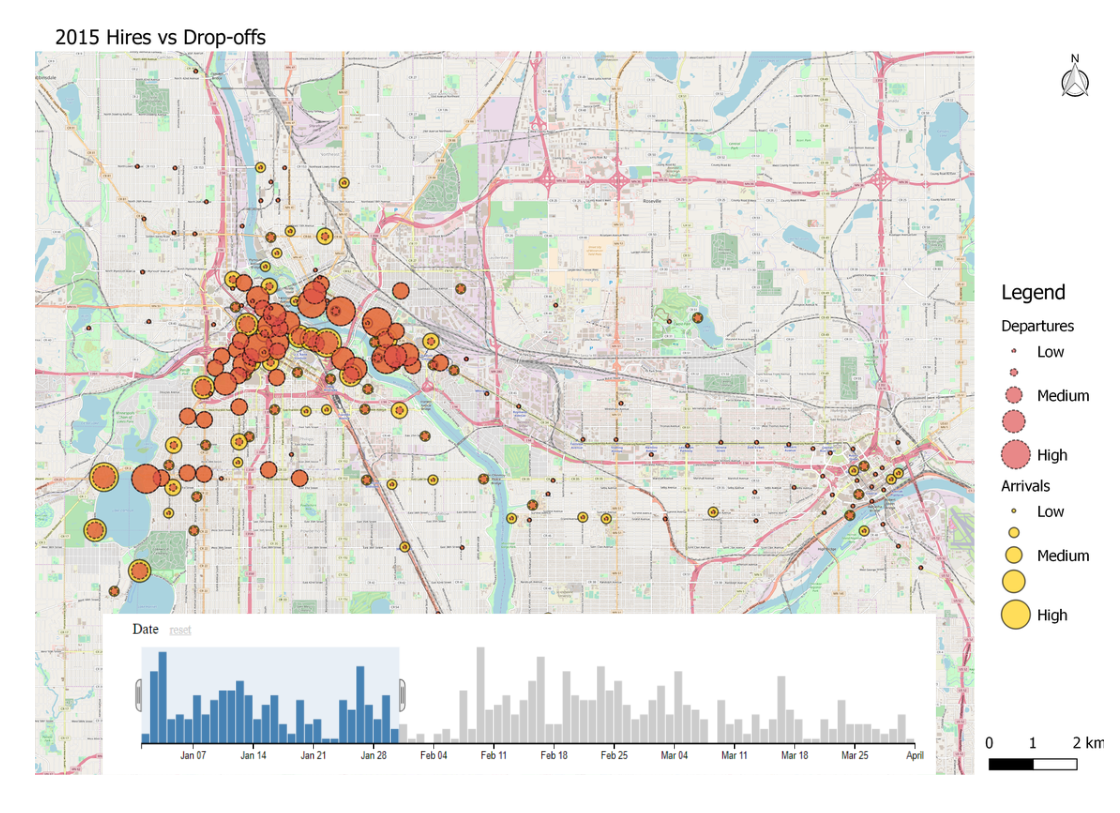
\includegraphics[scale=0.35]{figs/third_viz.PNG}
	\caption{\footnotesize{Crossfilter Enabled Mapping}}
	\label{fig:Third viz Chart}
	\captionsetup{justification=centering,margin=1cm}
	\vspace{-10pt}
\end{figure}

\subsection{Chosen Design}
\label{sec:viz4}

After considering all three visualizations based on their effectiveness, ease-of-use, complexity, and user-friendly interface, we decided to choose the third visualization \textbf{Crossfilter Enabled Geographic Mapping} as our chosen design. This visualization incorporated a number of different task abstractions viz. \textbf{comparison} between stations, \textbf{discover} trip duration in the histogram and maybe even \textbf{identify} outlier stations. This kind of visualization can be thought of as a focus + context design. When a certain area of time is highlighted, the remaining histogram greys out to denote that it is not included in the filter. Such design choices increase the effectiveness of the visualization. We also believe that using the real-time filter will adhere more to test volunteers who will find the visualization more interactive. Since users testing is a major part of our evaluation process, this result should definitely be taken in a positive vein.